\documentclass[dvisvgm, tikz, border=4pt]{standalone}
\begin{document}
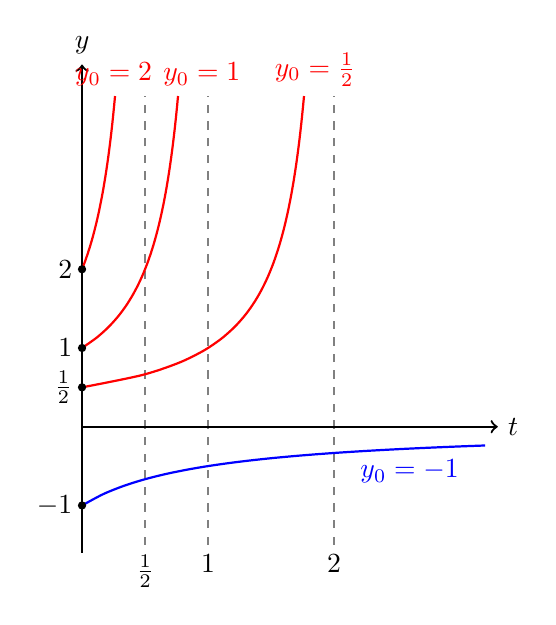
\begin{tikzpicture}[x=1.6cm,y=1cm]

  % Axes
  \draw[->,thick] (0,0) -- (3.3,0) node[right] {$t$};
  \draw[->,thick] (0,-1.6) -- (0,4.6) node[above] {$y$};

  % Blow-up times t* = 1/y0
  \draw[dashed,gray] (0.5,-1.5) -- (0.5,4.2);
  \draw[dashed,gray] (1,-1.5) -- (1,4.2);
  \draw[dashed,gray] (2,-1.5) -- (2,4.2);
  \node[below] at (0.5,-1.5) {$\frac12$};
  \node[below] at (1,-1.5) {$1$};
  \node[below] at (2,-1.5) {$2$};
  
  % y0 = 2: blows up at t = 1/2
  \draw[red,thick,domain=2:4.2,samples=25,smooth]
    plot ({0.5-1/\x},\x);

  % y0 = 1: blows up at t = 1
  \draw[red,thick,domain=1:4.2,samples=25,smooth]
    plot ({1-1/\x},\x);

  % y0 = 1/2: blows up at t = 2
  \draw[red,thick,domain=0.5:4.2,samples=25,smooth]
    plot ({2-1/\x},\x);

  % y0 = 0: stays at zero
  \draw[black,thick] (0,0) -- (3.2,0);

  % y0 = -1: decays to zero
  \draw[blue,thick,domain=0:3.2,samples=20,smooth]
    plot (\x,{-1/(1+\x)});

  % Initial values
  \foreach \y/\lab in {2/2, 1/1, 0.5/\frac12, -1/-1}{
    \fill (0,\y) circle (1.5pt);
    \node[left] at (0,\y) {$\lab$};
  }

  % Curve labels
  \node[red,above] at (0.25,4.2) {$y_0=2$};
  \node[red,above] at (0.95,4.2) {$y_0=1$};
  \node[red,above] at (1.85,4.2) {$y_0=\frac12$};
  \node[blue,below] at (2.6,-0.3) {$y_0=-1$};

\end{tikzpicture}
\end{document}
